\documentclass{article}
\usepackage{amsmath, graphicx}
\graphicspath{ {./images/} }

\title{Ch. 4 CW Pt. 2 Solns}
\author{Mr. Spence}
\date{\today}

\begin{document}

\maketitle

\begin{enumerate}

\item People's taste for oranges will increase after the discovery about diabetes, so the demand curve will shift right. The new fertilizer is a technological advancement that will shift the supply curve right. After the two shifts, the equilibrium quantity will unambiguously increase, but the change in equilibrium price is ambiguous.

	\begin{figure}[h]
	\centering
	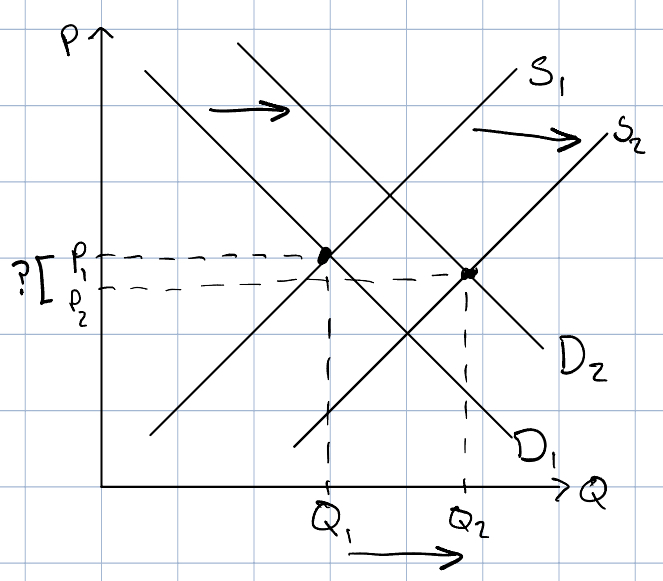
\includegraphics[width = 0.5\textwidth]{problem1}
	\end{figure}
	
\newpage
	
\item

	\begin{enumerate}
	
	\item A fall in the price of flour could be responsible. Since flour is an input to bagels, a fall in the price causes the supply of bagels to shift right. That increases the equilibrium quantity and decreases the equilibrium price of bagels. Since bagels and cream cheese are complements, a decrease in the price of bagels causes the demand for cream cheese to shift right. That increases the price of cream cheese.
	
	\begin{figure}[h]
	\centering
	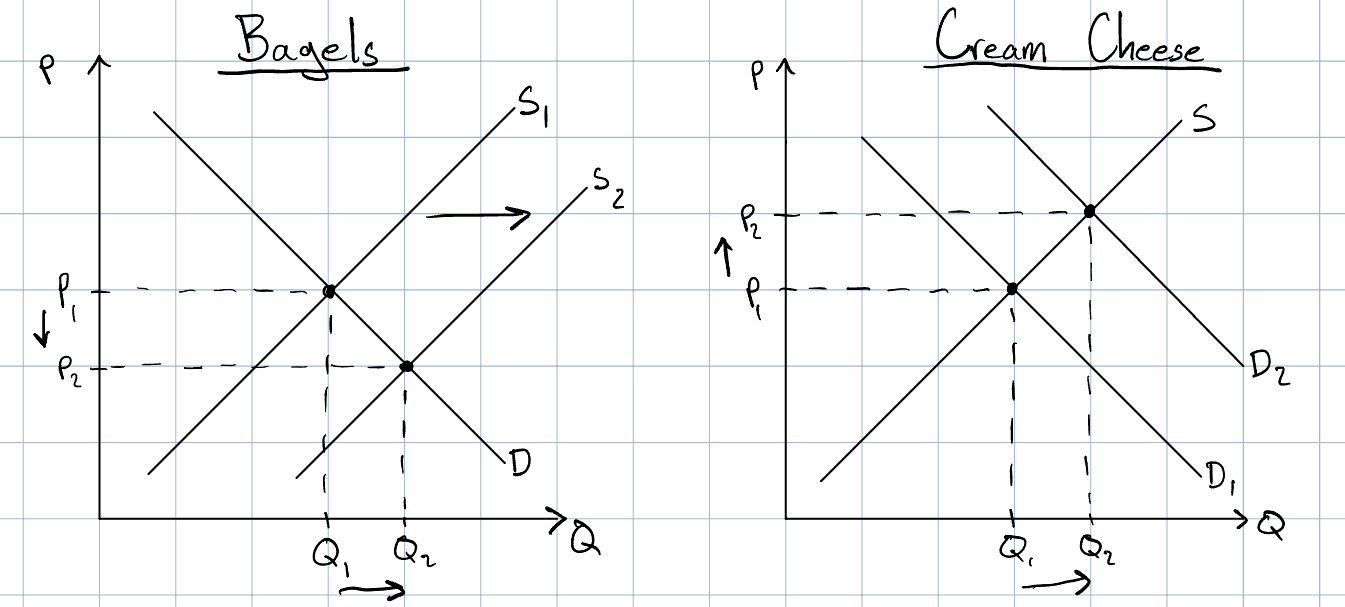
\includegraphics[width = \textwidth]{problem2a}
	\end{figure}
	
	\item A rise in the price of milk could be responsible. Since milk is an input to cream cheese, an increase in price causes the demand for cream cheese to shift left. That increases the equilibrium price of cream cheese. Since cream cheese and bagels are complements, an increase in the price of cream cheese causes the demand for bagels to shift left. That decreases the equilibrium quantity of bagels.
	
	\begin{figure}[h]
	\centering
	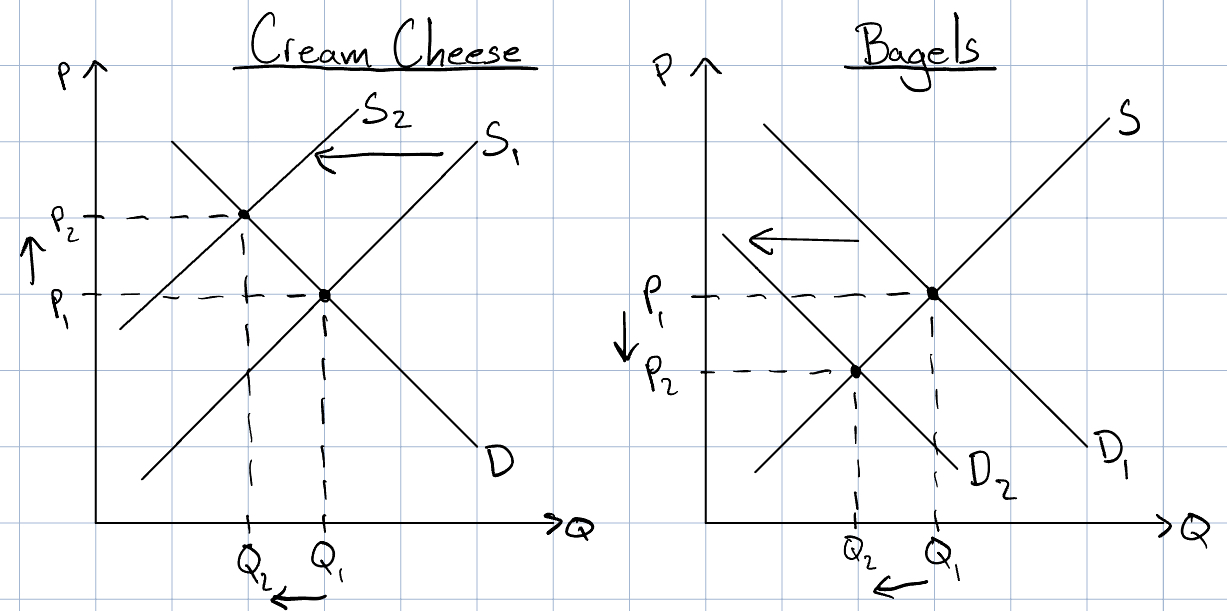
\includegraphics[width = \textwidth]{problem2b}
	\end{figure}
	
	\end{enumerate}
	
\newpage
	
\item

	\begin{enumerate}
	
	\item The supply curve is vertical which might be because the number of seats in the baseball stadium is fixed.
	
	\item $P^* = 8$ and $Q^* = 8,000$.
	
	\item 
	
	\begin{center}
	\begin{tabular}{c c c}
	\textbf{Price} & \textbf{Quantity Demanded} & \textbf{Quantity Supplied} \\
	\hline
	\$4 & 10,000 + 4,000  = 14,000 tickets & 8,000 tickets \\
	8 & 8,000 + 3,000  = 11,000 & 8,000 \\
	12 & 6,000  + 2,000 = 8,000 & 8,000 \\
	16 & 4,000 + 1,000 = 5,000 & 8,000 \\
	20 & 2,000 + 0 = 2,000 & 8,000
	\end{tabular}
	\end{center}
	
	$P^* = 12$ and $Q^* = 8,000$
	
	\end{enumerate}
	
\item

	\begin{enumerate}
	
	\item
	\begin{align*}
	Q_S &= Q_D \\
	4P^* &= 30 - 2P^* \\
	6P^* &= 30 \\
	P^* &= 5 \\
	\end{align*}
	
	\item
	\begin{align*}
	Q^* &= 4P^* \\
	Q^* &= 20
	\end{align*}
	
	\end{enumerate}
	
\item
	\begin{enumerate}
	
	\item
	\begin{gather*}
	Q_D = Q_S \\
	144 - 12P^* = 16 + 4P^* \\
	160 = 16P^* \\
	10 = P^* \\
	Q^* = 16 + 4P^* \\
	Q^* = 16 + 4(10) \\
	Q^* = 56
	\end{gather*}
	
	\item First, we need to calculate foreign demand before the increase:

	\begin{align*}
	Q_D &= Q_{D,Dom} + Q_{D,For} \\
	144 - 12 P &= 80 - 8P + Q_{D,For} \\
	64 - 4P &= Q_{D,For}
	\end{align*}
	
	Next, we need to calculate market demand after the increase in foreign demand:
	\begin{align*}
	Q_D' &= Q_{D,Dom} + 1.5Q_{D,For} \\
	Q_D' &= 80 - 8P + 1.5(64 - 4P) \\
	Q_D' &= 80 - 8P + 96 - 6P \\
	Q_D' &= 176 - 14P
	\end{align*}
	\end{enumerate}
	
	Now, we can calculate the equilibrium price:
	\begin{align*}
	Q_D' &= Q_S \\
	176 - 14P' &= 16 + 4P' \\
	160 &= 18P' \\
	\frac{80}{9} &= P'
	\end{align*}
	
\end{enumerate}

\end{document}